\section{Introduction}
\label{sec:introduction}

Research has historically been constrained by the number, ability, and organization
of human researchers. Artificial intelligence may relax this constraint. The
relevant change would not occur when AI becomes useful in ordinary production, or
even when it automates a large share of existing jobs. It would occur when AI systems
can perform the research tasks required to produce better AI systems. At that point,
AI capability would become an input into its own law of motion, and innovation would
no longer be tied mechanically to the supply of human researchers.

The paper does not model the earlier transition from an economy without commercially
useful AI to one that uses AI in ordinary production. One can think of that
pre-AI period as an economy with conventional production and human research, in
which scientific knowledge, algorithms, and computing capacity accumulate before AI
services become economically useful. A formal model of that transition would require
an adoption margin and an explanation of how research is financed before it produces
current AI revenues. We instead begin after productive AI services already exist but
while frontier research remains primarily dependent on human researchers. The object
of the paper is the subsequent automation of AI research.

\subsection{Why the transition matters}

The central economic question is not only whether AI raises output. It is whether
automating the production of better AI changes the constraints that have historically
kept technological progress on a balanced-growth path. While research remains human
intensive, the research workforce cannot grow persistently faster than population.
Automated research relaxes that constraint because additional output can finance
additional research services, which improve capability and expand output again. The
model determines when diminishing returns absorb this feedback and when the economy
instead enters an acceleration regime. It also shows why finite-scale observations
need not identify the asymptotic regime: when the production elasticity is close to
one, the relative-price threshold at which the gross-substitution force becomes
quantitatively important can be extremely large.

The distributional question is different from the growth question. A decline in
labor's share of output does not imply that the real wage falls, because productivity
and capital deepening can raise output per worker. Humans may therefore receive a
smaller share of a much larger economy while their wage rises. The ownership of
capital and monopoly rents then becomes central to the distribution of the gains.
The baseline assigns those rents to the representative household and consequently
does not model wealth concentration; this assumption mutes, rather than resolves,
the ownership question. The model also distinguishes the human intensity of AI
research from the number of humans it employs. The ratio $H/M$ can fall while the
employment share $H/N$ rises if the expansion of the research industry outweighs
the reduction in humans required per unit of automated research.

Market structure affects both the current and future uses of AI. A monopolist
restricts current deployment, but its operating rents give frontier improvements a
private value. Regulating the access price can therefore raise current production
while reducing the return to research unless policy replaces the lost innovation
incentive. The return to capital supplies another intertemporal margin. When
$\sigma_{XL}>1$ and capability is unbounded, output eventually expands faster than
capital and the marginal return rises without bound, so the usual stationary return
that supports balanced growth disappears.

This production-side mechanism is not the only route to acceleration. Even when
both substitution elasticities equal one, the feedback from capability to output,
from output to automated research, and from research back to capability can offset
diminishing returns. Under the proportional-allocation counterfactual studied below,
an exact balance makes the capability growth rate increase without bound, and
stronger feedback produces a finite-time singularity. The production elasticity and
the strength of recursive research feedback must therefore be treated as separate
dimensions.

A capital-deepening benchmark isolates what this conclusion does and does not require.
Replace AI services with a second reproducible capital service, allocate a constant
fraction of the capital stock to each of its two production uses, and save a constant
share of output. Gross substitution can then make labor asymptotically inessential,
but the production function becomes linear in total capital and the economy converges
at most to an $AK$ balanced-growth path. The growth rate does not increase without
bound. The additional feedback in our model comes from capability: better AI reduces
the resource cost of AI services and also enters the production of further capability.
The benchmark also shows that a vanishing labor share together with a rising wage is
not unique to AI. Our contribution concerns how this distributional outcome interacts
with recursive research, market power, and the transition between growth regimes.

These mechanisms are economically important but do not constitute a complete theory
of whether advanced AI benefits humanity. The present model contains no agency
failure, misalignment, existential damage, political power, or heterogeneous
ownership of AI rents. It characterizes the growth, factor-income, employment, and
market-structure conditions that a broader welfare analysis would need. It does not
assign a probability to transformative AI or establish that an acceleration regime
would be socially desirable.

\subsection{Empirical motivation}

The data do not yet measure the object at the center of the model: the share of AI
research performed by AI systems rather than humans. They do, however, reveal three
parts of the mechanism. The physical resources devoted to AI are expanding, the
quality-adjusted output obtained from those resources is growing even faster, and AI
systems can complete increasingly long tasks with less human intervention. These are
descriptive facts, not estimates of either substitution elasticity in the model.

\citet{korinekmckelvey2026} construct annual estimates of U.S. AI production using
compute expenditure, the stock of H100-equivalent processors, hardware performance,
and benchmark quality. Between 2023 and 2025, nominal compute expenditure rises from
\$36.9 billion to \$219.2 billion and raw compute capacity from 1.09 million to 10.7
million H100 equivalents. Their quality-adjusted inference index increases by a
factor of about 1,502 and their quality-adjusted training index by a factor of about
78. These last two quantities are model-based estimates assembled from sparse data
and explicit allocation assumptions; they should not be read as national-account
aggregates. Their economic value is the distinction they draw between installing
more compute and obtaining more services from each unit of compute. In the language
of our model, raw capacity is an input that can be allocated to inference or
research, quality-adjusted inference is closest to current AI services, and
quality-adjusted training is an imperfect proxy for the production of model capital.

The longer-run evidence points in the same direction. The compute used to train
notable models grew by a factor of approximately 4.1 per year between 2010 and May
2024; for recent frontier models, the estimated factor was approximately 4.2 per
year \citep{sevillaroldan2024}. The Stanford AI Index estimates that global AI
compute capacity grew by a factor of 3.3 per year between 2022 and 2025 and reached
17.1 million H100-equivalent units in 2025 \citep{stanfordaiindex2026}. None of these
series reveals how compute is divided between deployment and research or how much
human research it replaces.

\begin{figure}[htbp]
    \centering
    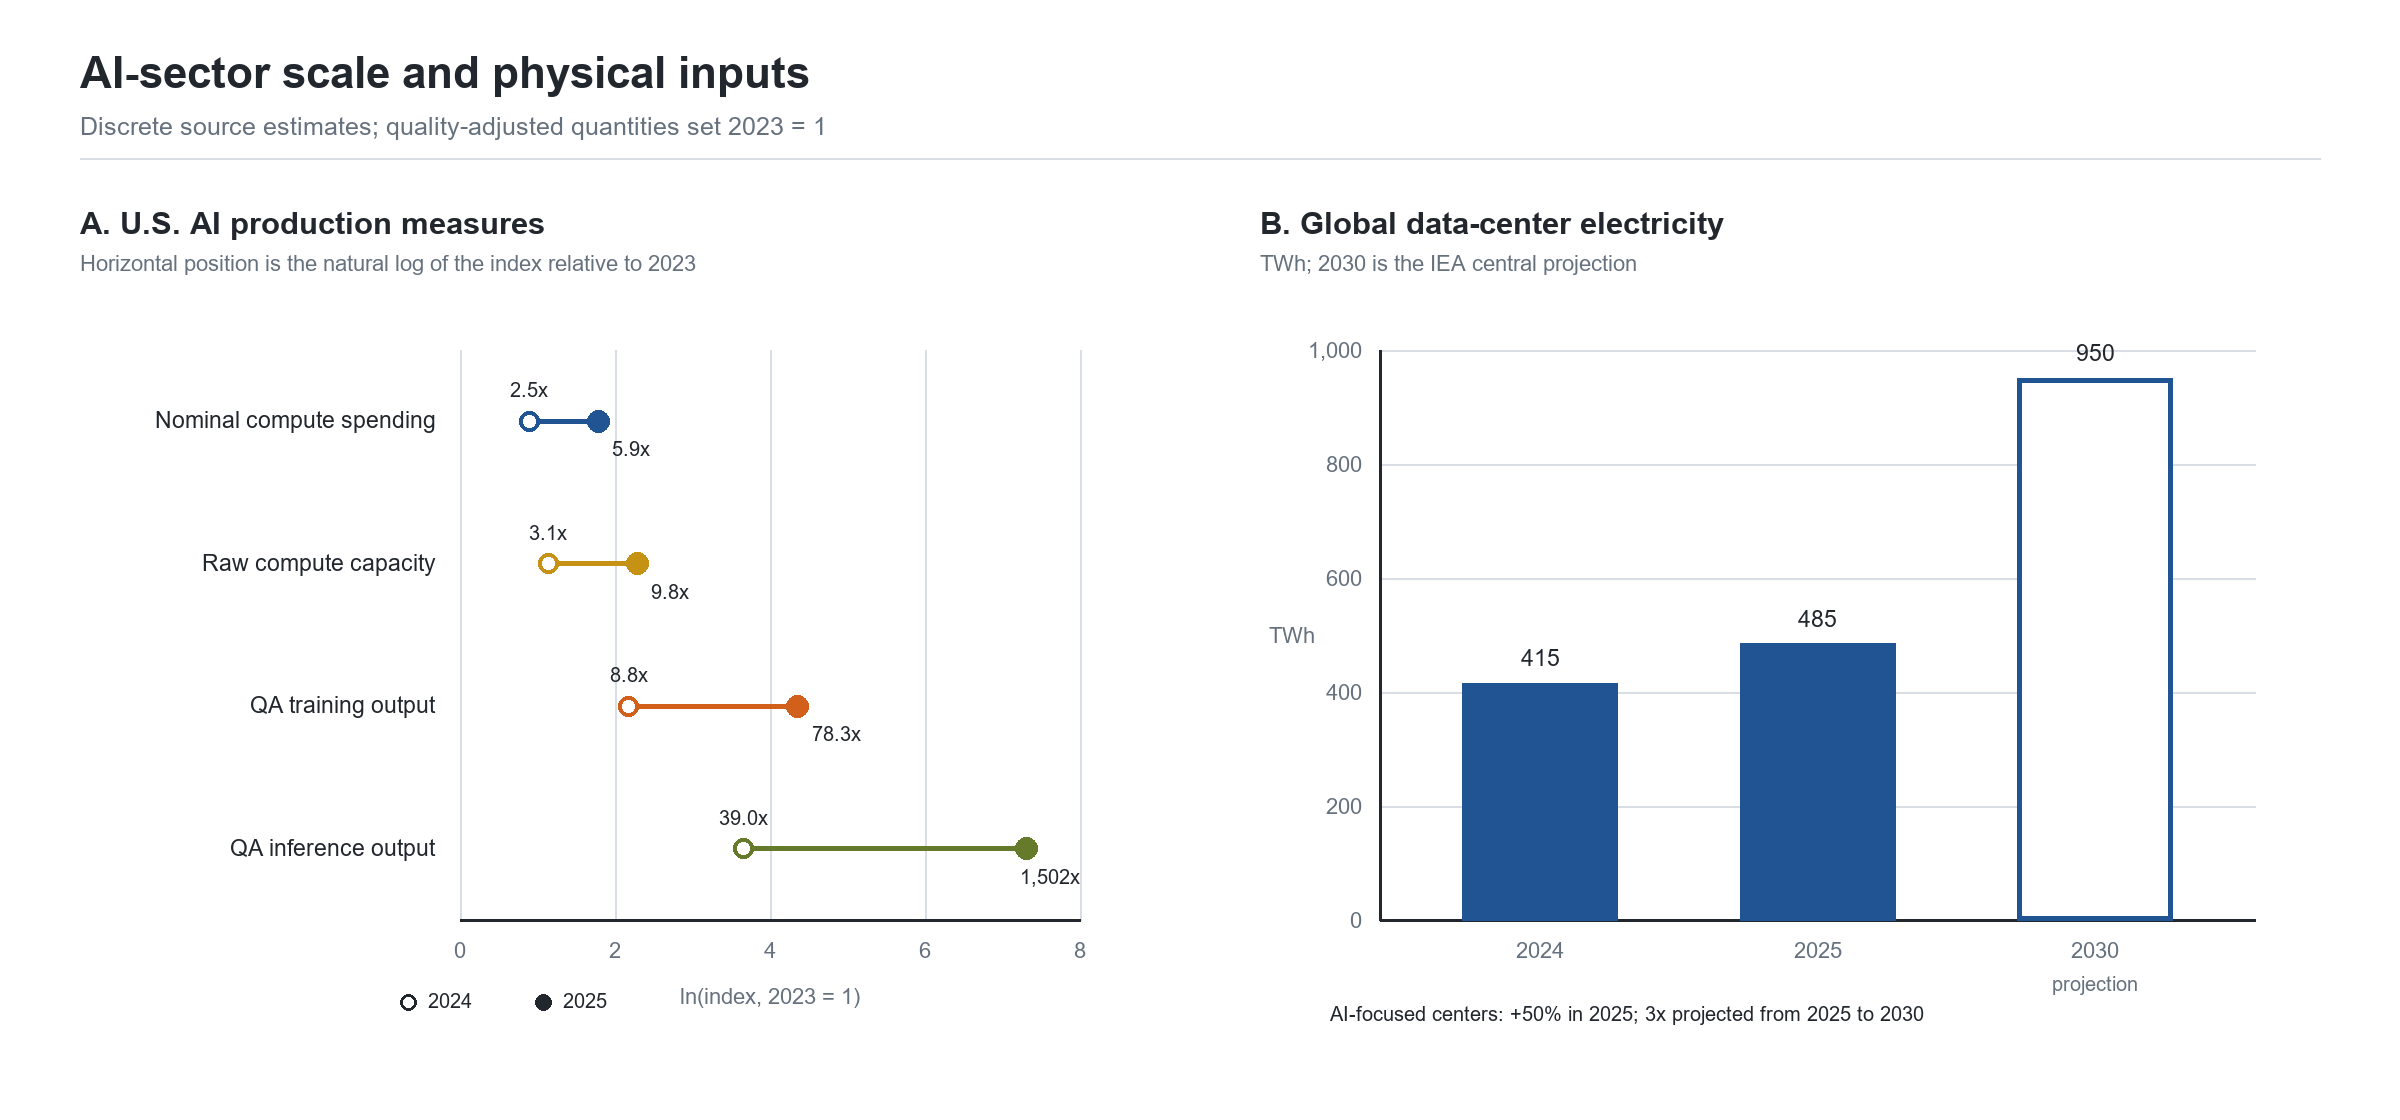
\includegraphics[width=\textwidth]{figures/empirical_ai_scale.png}
    \caption{AI-sector scale and physical inputs. Panel A reports discrete U.S.
    estimates for 2024 and 2025 relative to 2023; horizontal positions use the
    natural logarithm because the quality-adjusted quantities span several orders
    of magnitude. Panel B reports observed global data-center electricity use in
    2024 and 2025 and the IEA central projection for 2030. Sources:
    \citet{korinekmckelvey2026}, \citet{iea2025}, and \citet{iea2026}.}
    \label{fig:empirical-ai-scale}
\end{figure}

The cost of obtaining quality-adjusted AI services has fallen at the same time. The
lowest observed price for querying a model that reached the GPT-3.5 performance
level on MMLU fell from \$20 per million tokens in November 2022 to \$0.07 in October
2024. Over a similar period, the AI Index reports annual declines of 30 percent in
hardware costs and annual improvements of 40 percent in energy efficiency
\citep{stanfordaiindex2025}. This motivates our separation of raw inference compute
from quality-adjusted AI services. It does not identify AI capability separately: a
lower quality-adjusted price can reflect better algorithms, hardware, utilization,
or a lower markup.

Compute remains a real resource rather than a freely reproducible unit of
intelligence. Global electricity consumption by data centers rose from 415 TWh in
2024 to 485 TWh in 2025, while consumption at AI-focused facilities increased by 50
percent. The International Energy Agency projects total data-center consumption of
approximately 950 TWh in 2030 and a tripling of consumption at AI-focused facilities
between 2025 and 2030 \citep{iea2025,iea2026}. Figure
\ref{fig:empirical-ai-scale} therefore combines a rapid expansion in output with a
rapid, but much smaller, expansion in a physical input. This pattern motivates the
model's common resource cost and the compute and electricity constraints reserved
for the extended model. The baseline cost normalization is an abstraction, not a
claim that the marginal cost of compute will remain constant.

A different set of measurements speaks to capability and use. METR defines a
model's 50-percent task horizon as the length of task---measured by the time a human
expert would require---at which an AI agent succeeds half of the time. Its public
suite covers software engineering, machine learning, and cybersecurity tasks. The
estimated horizon rises sharply across model releases, but it is not the amount of
time an AI system works autonomously, and METR cautions that estimates above 16
hours are unreliable with the current task suite \citep{metrtimehorizon2026}.
Platform use provides another imperfect signal. In Anthropic's samples of Claude.ai
conversations, the share classified as directive---a subset of automation---was 27
percent in January 2025, 39 percent in August, and 32 percent in November
\citep{anthropiceconomicindex2025,anthropiceconomicindex2026}. The non-monotonic path
is itself useful: capability growth does not translate mechanically into realized
delegation. These proprietary samples cover one platform and conversations rather
than production quantities.

\begin{figure}[H]
    \centering
    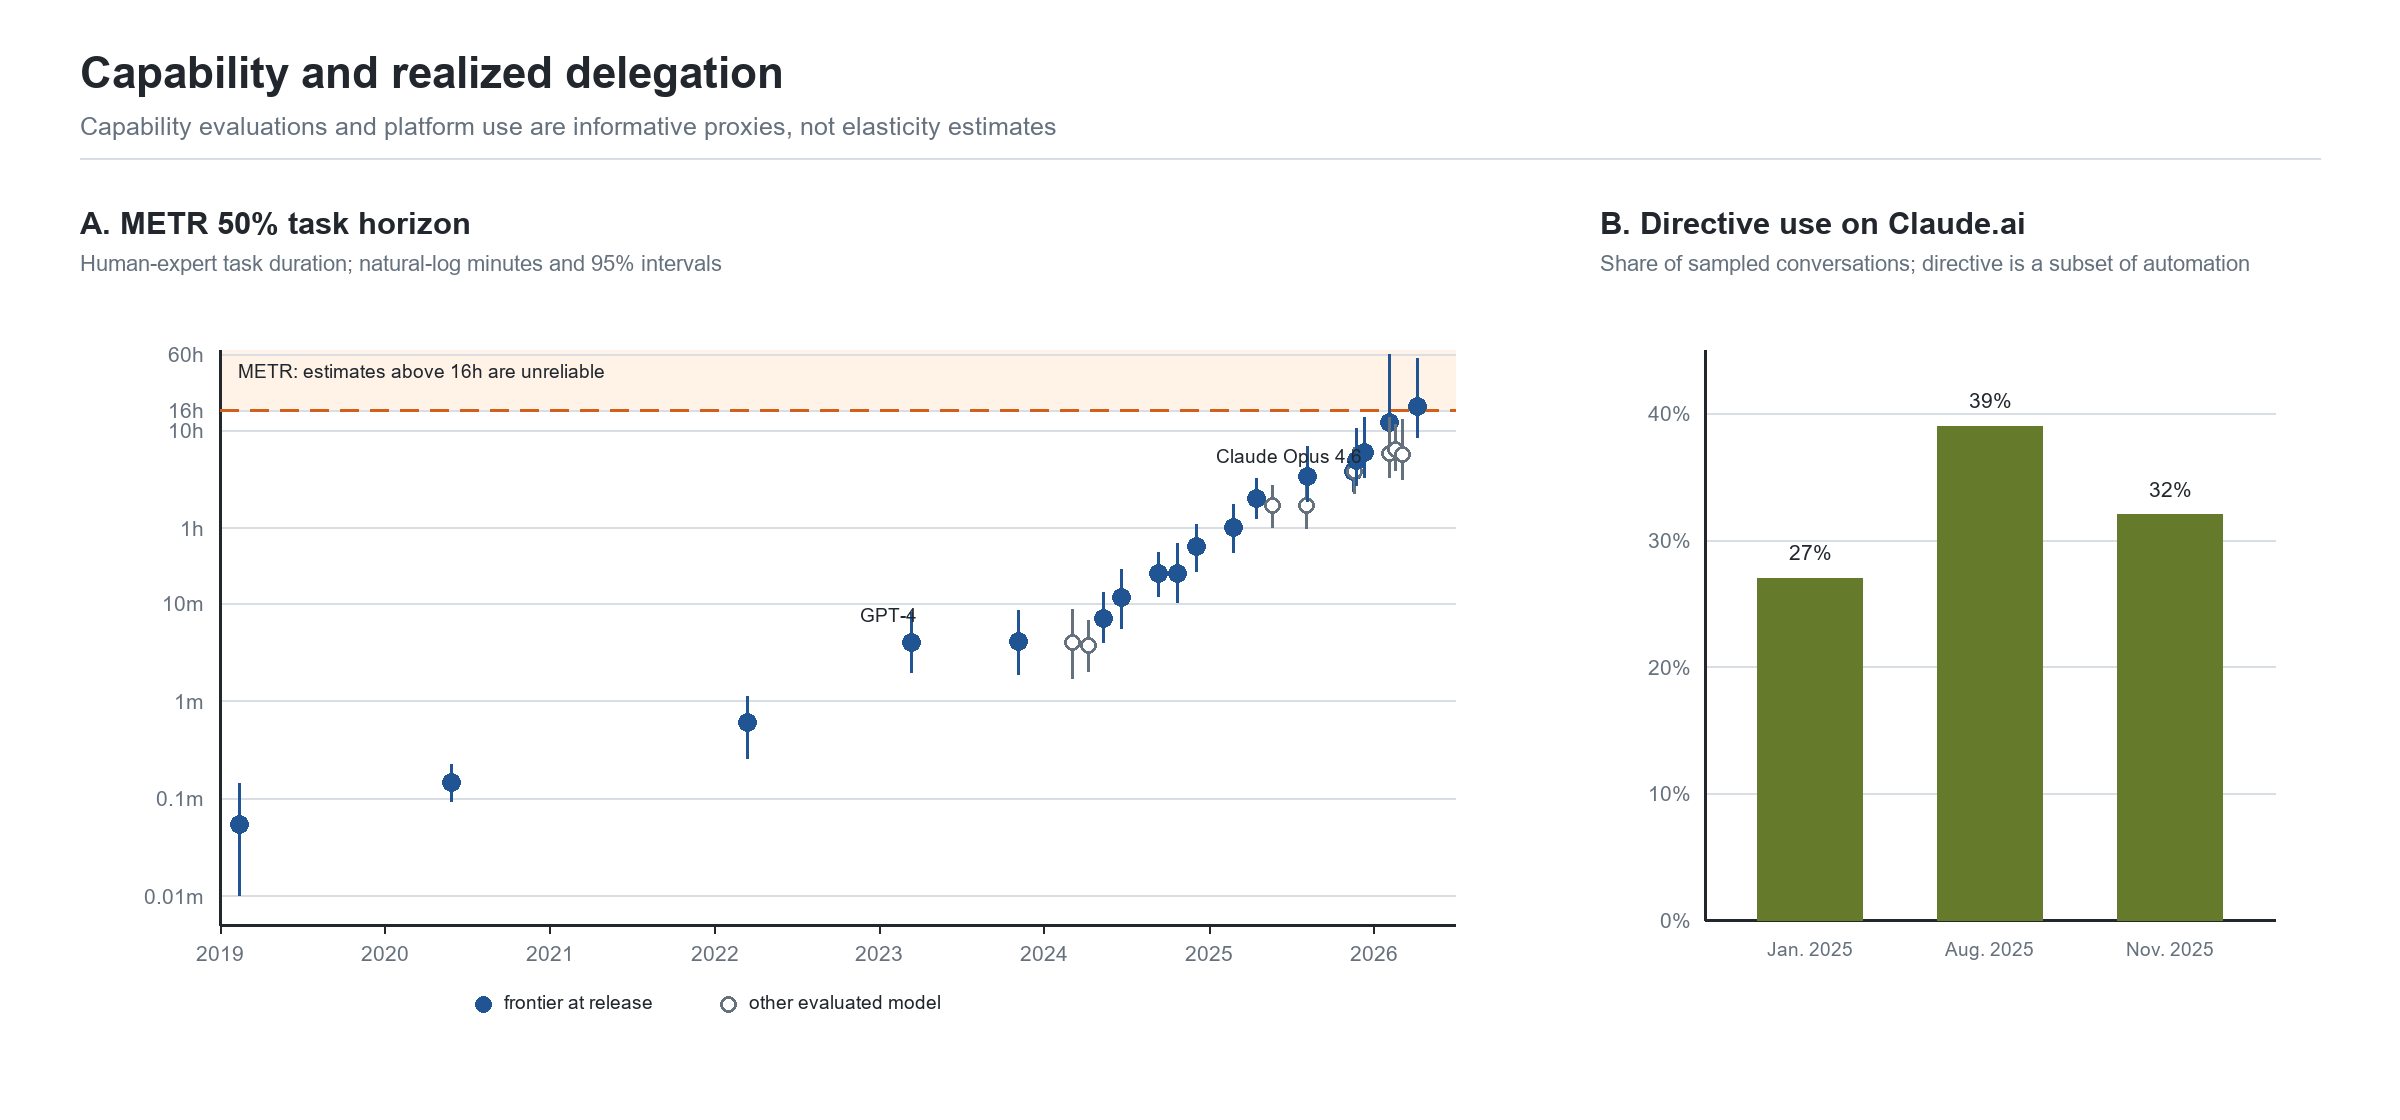
\includegraphics[width=\textwidth]{figures/empirical_automation_proxies.png}
    \caption{Capability and realized delegation. Panel A reports METR's estimated
    50-percent task horizon and 95-percent intervals for 26 evaluated models; the
    vertical scale is the natural logarithm of human-expert task minutes. The shaded
    region marks estimates above 16 hours, which METR regards as unreliable with the
    current task suite. Panel B reports directive use as a share of sampled Claude.ai
    conversations. Directive use is a subset of Anthropic's automation category.
    Sources: \citet{metrtimehorizon2026}, \citet{anthropiceconomicindex2025}, and
    \citet{anthropiceconomicindex2026}.}
    \label{fig:empirical-automation-proxies}
\end{figure}

Evidence closest to the automation of AI research comes from controlled evaluations,
not aggregate time series. In the original RE-Bench study, human experts given a
32-hour budget achieved almost twice the average score of the best AI agent on a set
of machine-learning research-engineering tasks \citep{metrrebench2024}. In a later
evaluation on a five-task subset, Claude 3.7 with a 32-hour budget matched the median
score of humans who had eight hours \citep{metrclaude2025}. This is evidence of a
changing frontier, but not a comparable two-date series: the model, scaffolding,
task subset, and time budgets differ. It therefore motivates the possibility that
automated research can substitute for human research without measuring the model's
human-to-machine research ratio.

Some striking internet statistics are less informative for our question. Cloudflare
reports that user-action crawler traffic rose by a factor of 21 during 2025 and that
AI bots accounted for an average of 4.2 percent of HTML page requests
\citep{cloudflareradar2025}. These are network requests, not tasks, workers, or value
added. We therefore do not treat bot traffic as evidence that AI has displaced human
labor.

Commercial scale has also increased. NVIDIA's data-center revenue rose from \$47.5
billion in fiscal year 2024 to \$115.2 billion in fiscal year 2025 and \$193.7
billion in fiscal year 2026 \citep{nvidia2026}. This is audited revenue from compute
hardware and networking, not total revenue from AI services. For frontier model
developers, the Stanford AI Index reports directional annualized-revenue estimates
of \$25 billion for OpenAI and \$19 billion for Anthropic around the beginning of
2026, while emphasizing differences in source quality and accounting definitions
\citep{stanfordaiindex2026}. The same report finds that industry produced more than
90 percent of notable models in 2025. These facts motivate a model in which private
demand, compute expenditure, and operating rents finance frontier research. They do
not establish monopoly or identify the markup earned by an integrated developer.

Taken together, the evidence motivates the model's state variables and the feedback
from AI services to AI research. It does not identify the substitution elasticity
between labor and AI services, the substitution elasticity between human and
automated research, or the probability of a singularity. We therefore do not use
these series to calibrate the transition. The numerical exercises discipline the
model's equilibrium logic; they are scenarios rather than forecasts.

\subsection{Economic mechanism and contribution}

This possibility raises an economic question before it raises a forecasting question.
Suppose frontier improvements combine human researchers and automated-research
services. Firms then choose both the scale and the composition of research. When the
research elasticity $\sigma_{HM}$ exceeds one, the two inputs are gross substitutes and
the automated share increases if the human research wage rises relative to the unit
resource cost of automated research. The conditional research-demand system
therefore represents automation as a continuous change in input composition rather
than as a date imposed on the model. Whether the equilibrium actually completes that
transition depends on the wage and automated-research-cost paths. Human researchers
can become asymptotically inessential, but substitution above one does not guarantee
that outcome: the wage must also rise relative to the cost of automated research.

Population growth is important during the human-dominated phase. In standard R\&D-based growth
models, new ideas depend on a growing but scarce human research input
\citep{romer1990,jones1995,aghionhowitt1992}. With diminishing returns to the stock of
ideas, a constant research-employment share implies semi-endogenous growth: the
long-run rate of innovation is pinned down by the growth of the research labor force.
Our benchmark preserves this logic while human research dominates. If population grows at rate
$n$, the capability growth rate is $\eta n/(1-\phi)$; without population growth,
positive asymptotic growth disappears when $\phi<1$.

Research automation can alter this result. Effective research labor can expand
through additional automated-research services rather than through population growth.
When those services dominate, capability growth is tied to their equilibrium growth
rate. Innovation can accelerate if higher output finances enough additional
automated research, but diminishing returns to ideas and research effort can preserve
a constant-growth path. The outcome depends separately on the production elasticity
$\sigma_{XL}$, the research elasticity $\sigma_{HM}$, and the allocation of output to research.

Human essentiality changes the strength of this feedback. Consider a counterfactual
in which research is Cobb--Douglas in human and automated inputs. Human research then
remains essential, and only the automated-input elasticity $\omega_M$ transmits the
feedback from output to research. Under Cobb--Douglas production, the human-essential
constant-growth candidate has a positive finite capability-growth rate only if
$1-\phi-\eta\omega_M\omega_X/\omega_L>0$. We maintain this restriction in the
baseline model and numerical experiments, but relax it in an analytical
counterfactual. Equivalently,
$\upsilon\equiv\beta/(1-\alpha-\beta)=\omega_X/\omega_L$. When automated research can instead become
asymptotically dominant, the condition becomes
$1-\phi-\eta\omega_X/\omega_L>0$. The second condition is stricter because $\omega_M<1$. There is
therefore a nonempty parameter region in which the human-essential candidate has
positive finite growth while the corresponding AI-dominated candidate does not.
Within the reduced proportional-allocation system, the sign of the human-essential
denominator also has an independent interpretation. A positive value produces a
stable positive growth rate, a zero value produces double-exponential capability,
and a negative value produces a finite-time singularity. The relevant threshold is
zero, not one.
This comparison is between two research technologies; it does not assume that the
research elasticity changes during the transition in the CES model. It is also
conditional on Cobb--Douglas production. If $\sigma_{XL}>1$ and capability is
unbounded, the output--capital ratio and the return to capital diverge. The household
Euler equation then makes consumption growth diverge, ruling out an interior steady
state with finite constant growth rates. This is a separate production-side
acceleration mechanism. Human essentiality weakens the research feedback but does
not by itself restore balanced growth.

The break at $\sigma_{XL}=1$ is asymptotic rather than a jump in finite allocations.
The exact CES share is continuous in the elasticity for every finite relative price,
but the limits in which $w/p^X$ becomes unbounded and the elasticity approaches one
do not commute. Under the high-capability regularity condition used below, unbounded
capability generates precisely this relative-price limit. Moreover, the relative-price threshold required for a given AI
share diverges exponentially in $1/(\sigma_{XL}-1)$. An elasticity just above one
can therefore produce an arbitrarily long quasi-Cobb--Douglas transition even though
its infinite-horizon regime has no finite constant-growth steady state.

The failure of the balanced-growth condition is not sufficient for a finite-time
singularity. Under the proportional-allocation closure used to isolate the feedback,
$D>0$ gives stable balanced growth, $D=0$ gives accelerating growth that remains
finite at every finite date, and a persistent $D<0$ produces a finite-time
singularity. During the CES transition, the relevant denominator is
$D(s^M_t)=1-\phi-\eta\upsilon s^M_t$. The automation share must cross the critical
value $(1-\phi)/(\eta\upsilon)$ and remain high long enough for the integral
condition derived below to be met. This distinction prevents the absence of a constant-growth path
from being interpreted mechanically as an immediate explosion.

Recent discussions often move too quickly from this mechanism to one of two
conclusions. One view treats an intelligence explosion as the natural implication of
automating AI research. The other assumes that physical bottlenecks and diminishing
returns will necessarily preserve familiar growth rates. Neither conclusion follows
without specifying the ideas production function. Scenario exercises such as
\citet{kokotajlo2025} make the feedback mechanism concrete, but rapid takeoff depends
on several jointly necessary assumptions about research automation, algorithmic
progress, compute, and organizational capacity. An economic model should expose those
assumptions separately.

Market structure determines both current use and the private return to innovation.
Frontier AI requires large fixed investments and may exhibit economies of scale and
scope \citep{korinekvipra2025,gans2024}. A monopolist restricts the current supply of
AI services but captures operating rents that raise the private value of better
capability. We therefore begin with one integrated developer that both supplies
quality-adjusted AI services and invests in the frontier. Competitive final-good
firms combine capital with a CES composite of production labor and AI services. The
production elasticity $\sigma_{XL}$ inside this composite governs adoption and the demand
elasticity faced by the monopolist.

The production elasticity $\sigma_{XL}$ separates the response of the real wage from the
response of the production-labor share. An expansion of AI services reduces this share when AI and
production labor are gross substitutes, but the wage falls only when substitution is
sufficiently strong. There is therefore an intermediate region in which production
workers receive a smaller share of output even though their wage rises. This
distinction is important for the distributional analysis: a declining labor share is
not, by itself, evidence that the real wage has fallen. In the full model, the
aggregate labor share also depends on how workers are reallocated between production
and research. An increase in the human-research employment share raises aggregate
labor income relative to production labor income; a decrease lowers it.
There is a sharper conditional result under Cobb--Douglas research and a fixed
automated-research spending share. The human-research wage bill is then a constant
share of output, so the production and aggregate labor-income shares rise together
when $\sigma_{XL}<1$ and remain constant when $\sigma_{XL}=1$. This result belongs
to a reduced allocation rule and is not used to characterize the numerical
equilibrium paths.

A separate distinction operates within the AI-development industry. The ratio
$H/M$ measures the human intensity of research, whereas $H/N$ measures the fraction
of the population employed as human researchers. Research can become less human
intensive while the development industry employs more people: $H/M$ falls when
automated research becomes cheaper relative to human research, but $H/N$ rises if
the scale of automated research per capita expands sufficiently quickly. The model
therefore allows an initial decline followed by an increase in human research
employment even along a path of continuous research automation.

The resulting welfare problem has two distinct margins. Static market power reduces
the current use of AI services. At the same time, consumer surplus and knowledge
spillovers imply that the developer may capture only part of the social value of
better AI and therefore invest too little in research. Reducing the markup can
correct the deployment distortion while also eroding the rents that finance
innovation. Price regulation and research policy must consequently be studied
together. The present version isolates this market-structure mechanism.

The six technology classes defined by $\sigma_{HM}\in\{1,>1\}$ and
$\sigma_{XL}\in\{<1,1,>1\}$ organize four groups of results. First, research automation is a
continuous equilibrium transition. Its speed depends on $\sigma_{HM}$ and on the
growth of the human research wage relative to the cost of automated research;
$\sigma_{HM}>1$ alone does not make the human contribution disappear. The same
conditions distinguish research composition from research employment: $H/M$ can
fall while $H/N$ rises.

Second, the model characterizes the feedback from research automation to growth.
Population growth sustains semi-endogenous capability growth while human research
dominates. If human and automated research are Cobb--Douglas, the essential human
input weakens the feedback from output to innovation. When automated research can
instead become asymptotically dominant, the stability condition is strictly more
demanding. The two candidate allocations identify a parameter region in which the
human-essential candidate has positive finite growth but the AI-dominated candidate
does not. Under
the reduced proportional-allocation closure, a positive value of the feedback denominator gives
constant growth, a zero denominator gives acceleration without finite-time
divergence, and a sufficiently persistent negative denominator gives a finite-time
singularity. With an endogenous automation share, a temporary crossing of the local
threshold is not sufficient; the accumulated feedback must reach the exact integral
condition derived below.
The fully Cobb--Douglas counterfactual makes the distinction especially transparent.
Even with unit substitution elasticities in production and research, an exact balance
between diminishing returns and the output--research feedback makes the capability
growth rate rise without bound. If the feedback is stronger, the reduced system
reaches a finite-time singularity. Explosive growth therefore does not require
$\sigma_{XL}>1$.

Third, the production elasticity creates a separate phase diagram. If
$\sigma_{XL}<1$, labor remains a bottleneck and any interior constant-growth limit
has zero per-capita output growth. In any nondegenerate limit that also satisfies the
developer's optimality conditions, human and automated research grow more slowly
than population and capability grows at rate $\eta n/(1-\phi+\eta)$. At
$\sigma_{XL}=1$, an AI-dominated positive constant-growth candidate requires the
stability and resource-feasibility restrictions. If
$\sigma_{XL}>1$ and capability is unbounded, the output--capital ratio and the return
to capital diverge, so the household Euler equation rules out an interior steady
state with finite constant growth rates. This remains true when human research is
essential. The discontinuity at one is a singular perturbation: finite allocations
are continuous in $\sigma_{XL}$, but the asymptotic limits do not commute and the
scale required for AI dominance diverges as $\sigma_{XL}\downarrow1$.

Fourth, the production structure separates factor-income outcomes. An expansion of
AI services lowers production labor's share when $\sigma_{XL}>1$, whereas its direct
effect raises the real wage when $\sigma_{XL}<1/\alpha$. Capital deepening and the
reallocation of workers between production and research determine the corresponding
general-equilibrium paths. The exact wage-growth decomposition identifies when
AI-services deepening works against wage growth, but the paper does not claim that
this force dominates without solving the associated equilibrium transition. The
aggregate labor share can also differ from the production-labor share because it
includes human researchers. Finally, monopoly creates a static deployment
distortion but also the rents that give frontier capability a private value; an
explicit social-value extension can create a distinct reason for private research to
remain below the social level. The baseline model does not sign that wedge.

The numerical section solves the decentralized perfect-foresight canonical system,
rather than fixing investment and research-spending shares. Under
$\sigma_{XL}=0.75$, output per capita falls initially, recovers, and then converges
toward a constant level while capability continues to grow. The production-labor
share rises as labor becomes the bottleneck. Under Cobb--Douglas production,
research automation is gradual: the automated contribution to research rises from
10.6 percent initially to 45.4 percent after 600 years and approaches one only over
a much longer horizon. Capability and per-capita output growth converge to their
analytical constant-growth values. Human research employment is non-monotone along
this path even though its long-run share of the population is zero.

A second Cobb--Douglas production path changes only the research elasticity from
$\sigma_{HM}=2$ to $\sigma_{HM}=1$. Human research then remains essential and its
share of the population converges to 0.497 percent. Capability growth converges to
1.738 percent rather than 2.274 percent, and per-capita output growth converges to
0.435 percent rather than 0.568 percent. Both paths satisfy the same canonical
equilibrium system. The comparison isolates how research substitutability changes
both the composition of research and the strength of recursive feedback.

For $\sigma_{XL}>1$, the numerical section uses the model's singular asymptotic
ratios rather than imposing a nonexistent finite-growth terminal state. Calendar
time to a large output--capital ratio is endogenous, and the boundary is moved
outward until the initial jump variables and the implied singularity date converge.
The common parameters keep both the human-essential and AI-dominated research
feedback denominators positive. The high-$\sigma_{XL}$ experiments therefore isolate
the production-side acceleration mechanism rather than the $D_{\mathrm{CD}}\leq0$
counterfactual.
For $\sigma_{XL}=1.35$, 1.50, and 2.00, the selected equilibrium branch remains close to moderate
growth for a long interval and then accelerates toward a finite-time singularity.
Higher substitution brings the acceleration forward. The wage rises throughout
all three paths, while the aggregate labor share approaches zero. These dates are
conditional numerical examples, not calibrated forecasts.

An additional search crosses the static wage threshold $1/\alpha$ and jointly
considers high production elasticities and faster population growth. These paths
satisfy the canonical equilibrium equations on their computed domains, but they
extrapolate the AI-dominated terminal boundary beyond the region established by the
analytical result. The computed wage can fall temporarily: with
$\sigma_{XL}=6.28$ and $n=3.9$ percent, its peak-to-trough decline is 9.39 percent.
The wage then recovers as capital accumulates and the movement of workers into AI
research makes production labor scarce. The wage at the trough remains 16.72 percent
above its initial level. This is a conditional numerical branch, not a proof that
every equilibrium with a high production elasticity eventually recovers.

Figure~\ref{fig:high-sigma-equilibrium-growth} previews this transition. It is
included here to show the quantitative object the paper seeks to explain, not as
evidence for the propositions. Section~\ref{sec:analytical-results} derives the
analytical foundations used across regimes. Section~\ref{sec:numerical} then
organizes the results into four cases and presents, within each case, the analytical
characterization and an equilibrium transition.

\begin{figure}[htbp]
    \centering
    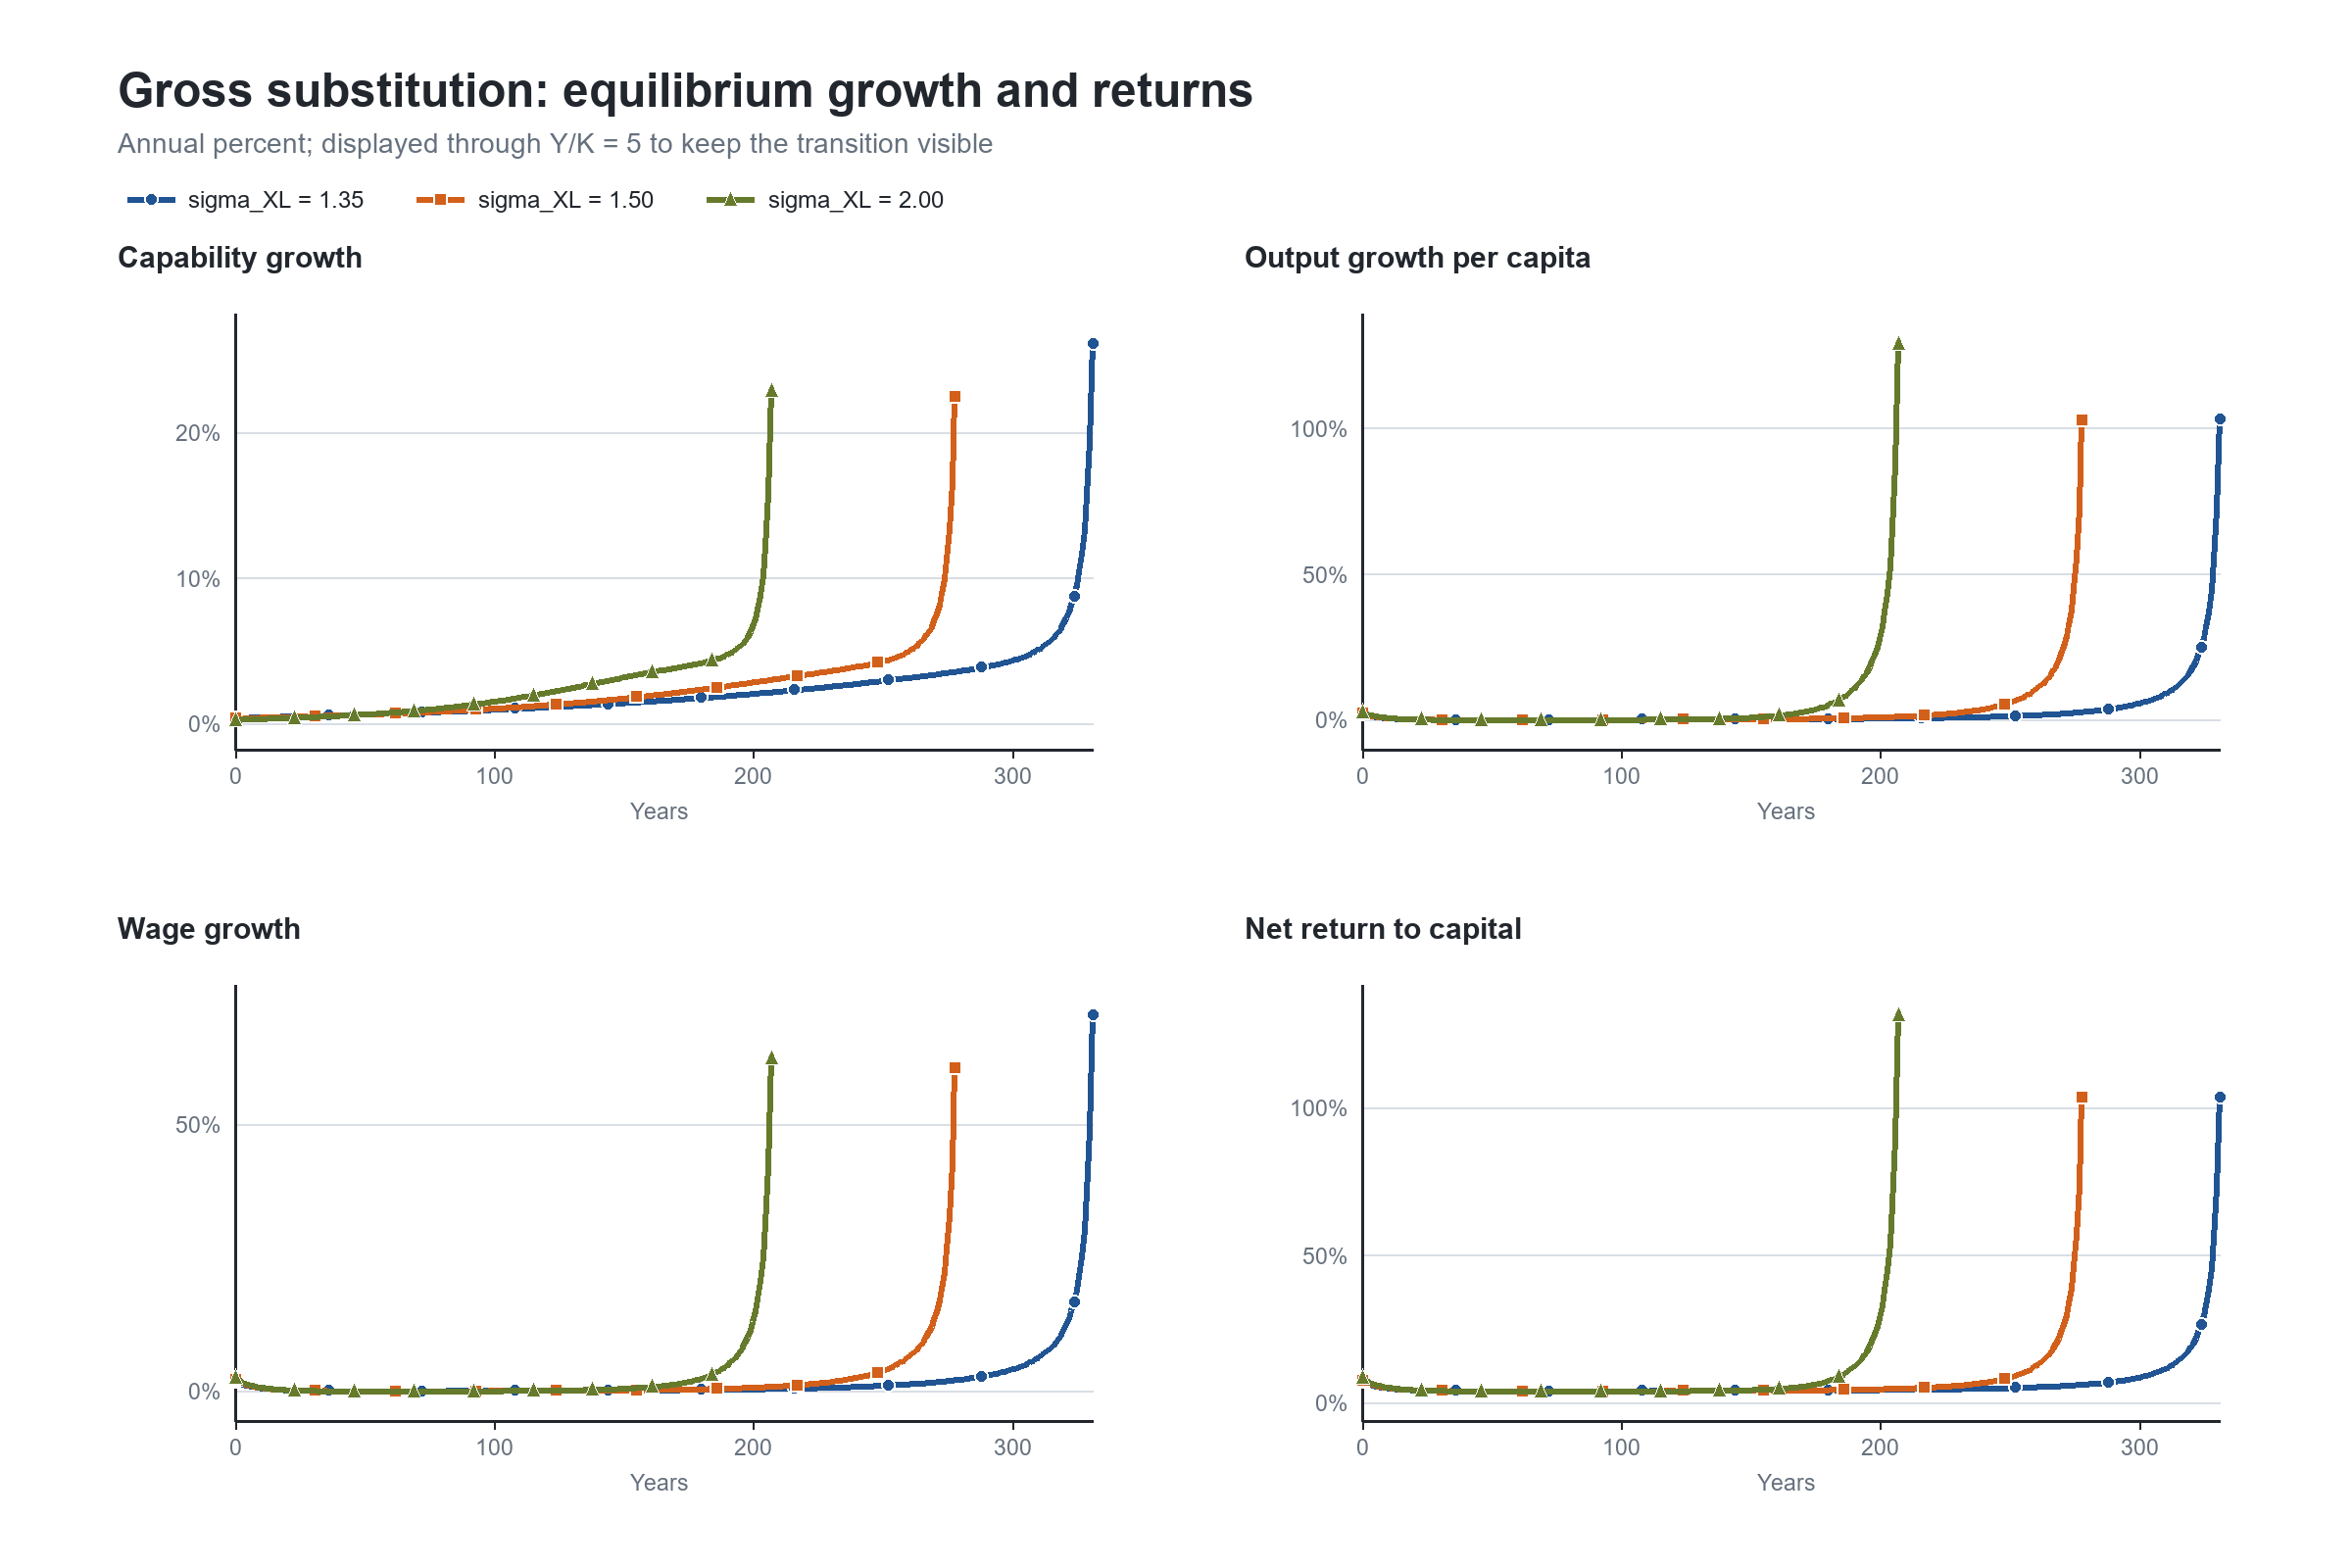
\includegraphics[width=\textwidth]{figures/high_sigma_equilibrium_growth.png}
    \caption{Preview of equilibrium growth rates and the net return under gross
    substitution. The figure stops at $Y/K=5$ to keep the pre-acceleration
    transition visible. The paths and their numerical validation are presented in
    Section~\ref{sec:numerical}.}
    \label{fig:high-sigma-equilibrium-growth}
\end{figure}

The extended model retains the integrated monopolist and adds distributional
heterogeneity and richer capital and compute accumulation. It will compare a
laissez-faire monopoly with regulated access prices, research subsidies or prizes,
and policies that combine both instruments. The objective is not to select a policy
before solving the model. It is to identify when lower AI-service prices must be
paired with explicit support for frontier research.

A task-based extension introduces task-specific AI productivity and fixed
automation costs. The extension makes the set of automated research tasks
endogenous and separates the intensive human--machine substitution margin from the
extensive margin on which new tasks become economical to automate. It also provides
a second reason for an initially small automated share: at low research scale, the
variable-cost savings from automation may not cover task-specific integration and
verification costs.

The rest of the paper is organized as follows. Section~\ref{sec:literature} relates
the framework to endogenous growth, transformative AI, automation and labor income,
measurement of AI services, and industrial organization. Section~\ref{sec:toy}
develops the baseline model and derives the analytical foundations.
Section~\ref{sec:numerical} studies four growth regimes. Each regime pairs the
relevant analytical result with an audited numerical equilibrium path.
Section~\ref{sec:extended} sets out the extended general-equilibrium model, and
Section~\ref{sec:task-extension} introduces research tasks and fixed automation
costs.
Section~\ref{sec:regulation} defines the regulatory scenarios.
Section~\ref{sec:conclusion} concludes.
